\chapter{Published Papers}

\subsubsection{Definitive Benchmark Study of Ring Current Effects on Amide Proton Chemical Shifts}
\underline{Anders S. Christensen}, Stephan P. A. Sauer, Jan H. Jensen (2011) Definitive benchmark study of ring current effects on amide proton chemical shifts. \textit{Journal of Chemical Theory and Computation}, 7:2078-2084.
\\\\ This paper describes our computational method to calculate ring current effects on amide proton chemical shifts using QM methods.
Furthermore, we compare three classical approximation to calculating ring-current effects in proteins, and find that they have similar performance.
When using the parameters set obtained here, the estimated error on the classically calculated ring-current effect on amide proton chemical shifts is less than 0.1 ppm.
\clearpage
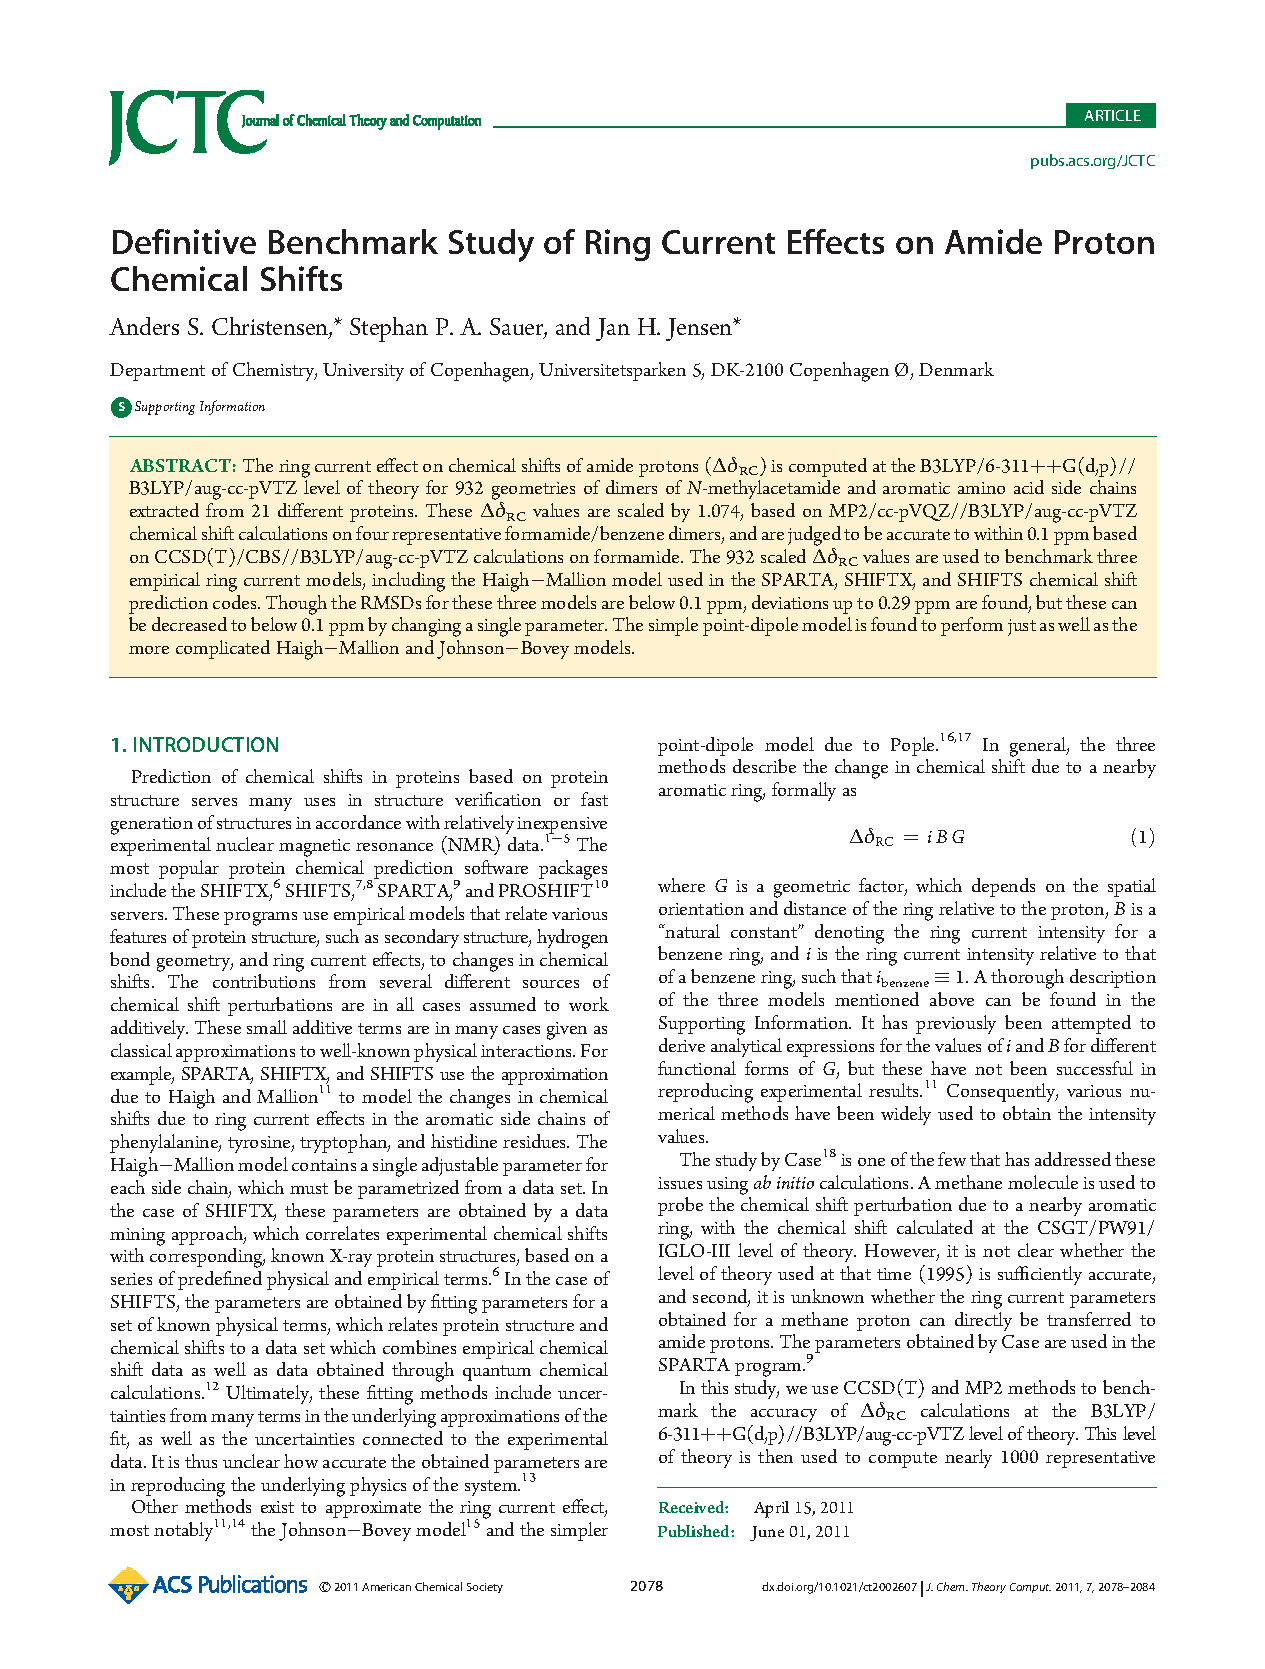
\includepdf[pages={1-7}]{papers/ct2002607.pdf}

\subsubsection{PHAISTOS: A Framework for Markov Chain Monte Carlo Simulation and Inference of Protein Structure}
Wouter Boomsma, Jes Frellsen, Tim Harder, Sandro Bottaro, Kristoffer E. Johansson, Pengfei Tian, Kasper Stovgaard, Christian Andreetta, Simon Olsson, Jan B. Valentin, Lubomir D. Antonov, \underline{Anders S. Christensen}, Mikael Borg, Jan H. Jensen, Kresten Lindorff-Larsen, Jesper Ferkinghoff-Borg, Thomas Hamelryck (2013) PHAISTOS: A framework for Markov chain Monte Carlo simulation and inference of protein structure. \textit{Journal of Computational Chemistry}, 34:1697-1705.
\\\\ In this paper, we describe the PHAISTOS program.
\clearpage
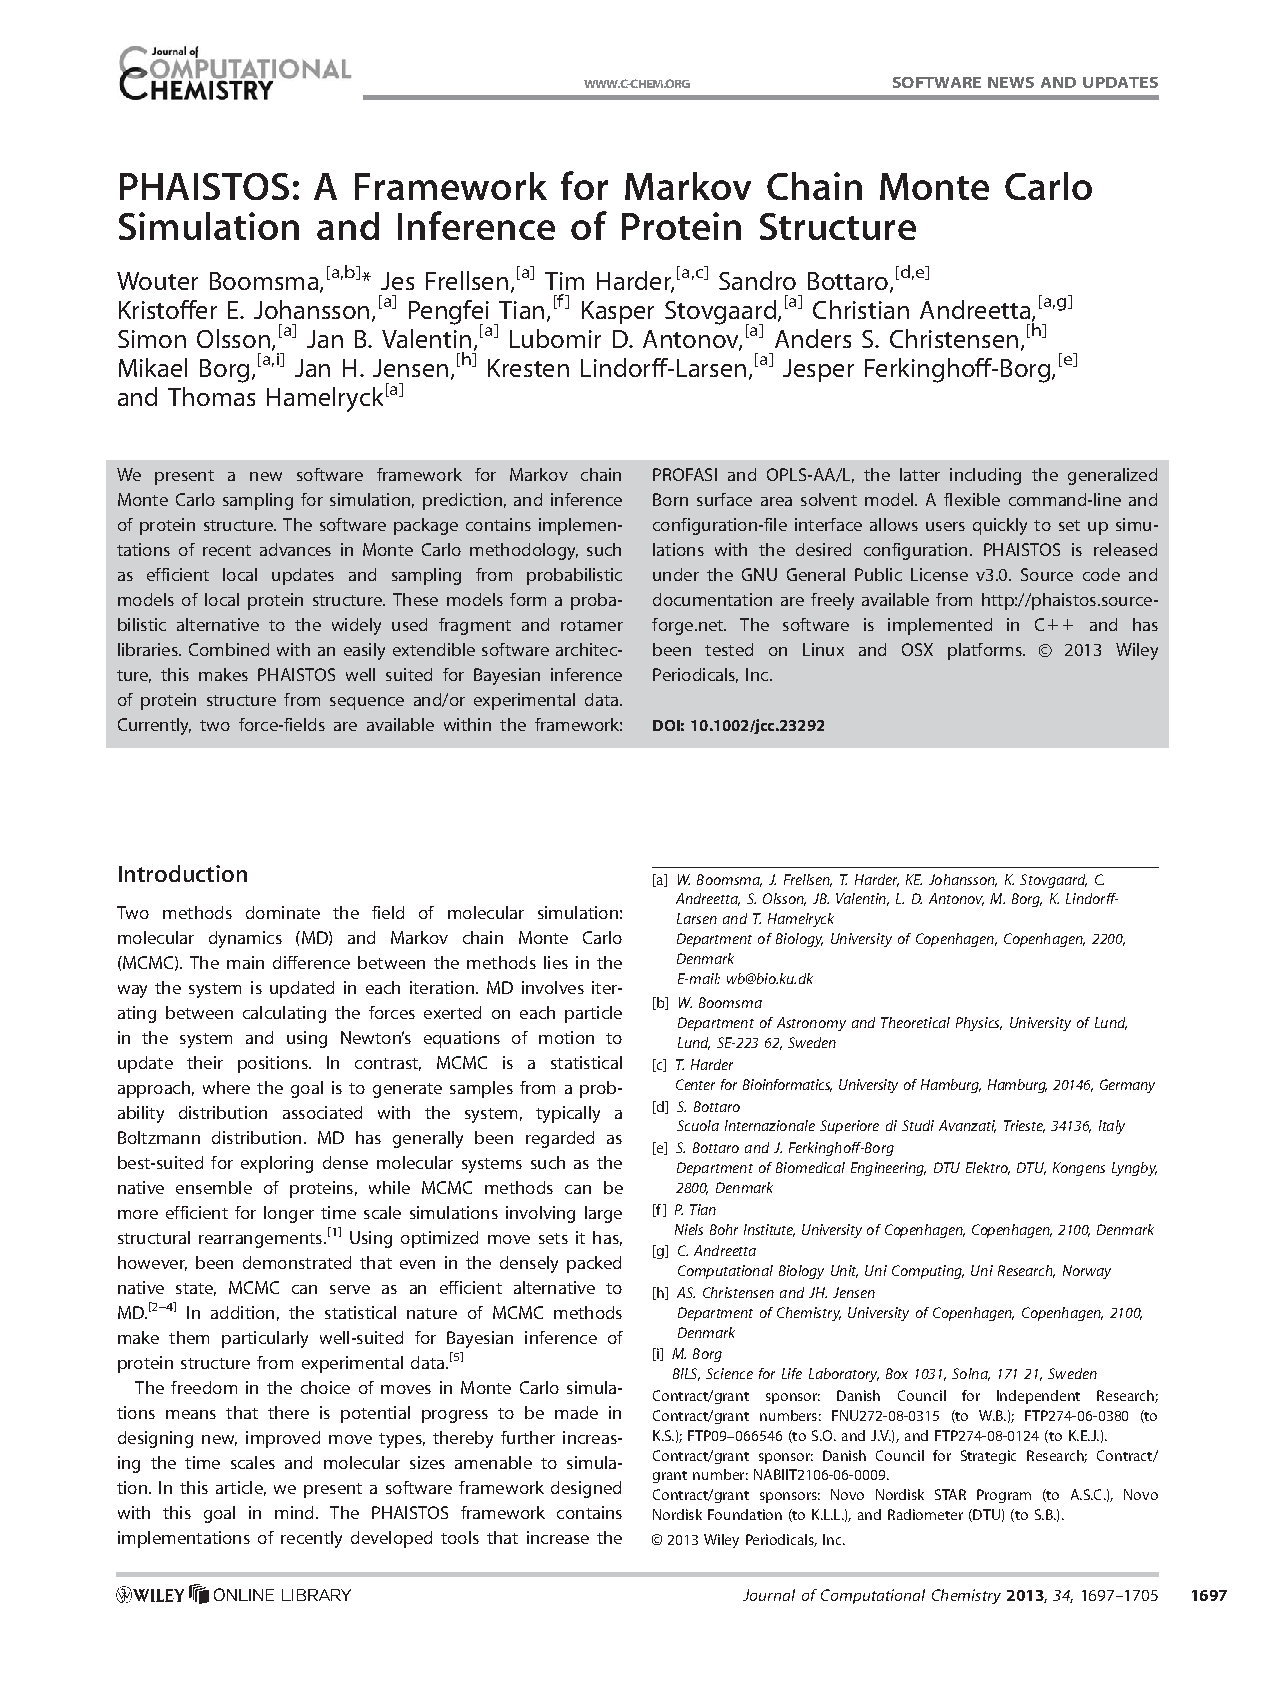
\includepdf[pages={1-9}]{papers/jcc23292.pdf}

\subsubsection{Protein Structure Validation and Refinement Using Amide Proton Chemical Shifts Derived from Quantum Mechanics}
\underline{Anders S. Christensen}, Troels E. Linnet, Mikael Borg, Wouter Boomsma, Kresten Lindorff-Larsen, Thomas Hamelryck, Jan H. Jensen (2013)  Protein Structure Validation and Refinement Using Amide Proton Chemical Shifts Derived from Quantum Mechanics. \textit{PLoS ONE} 8:e84123.
\\\\ In this paper, we demonstrate the accuracy of the QM-derive amide proton chemical shift predictor called ProCS.
\clearpage
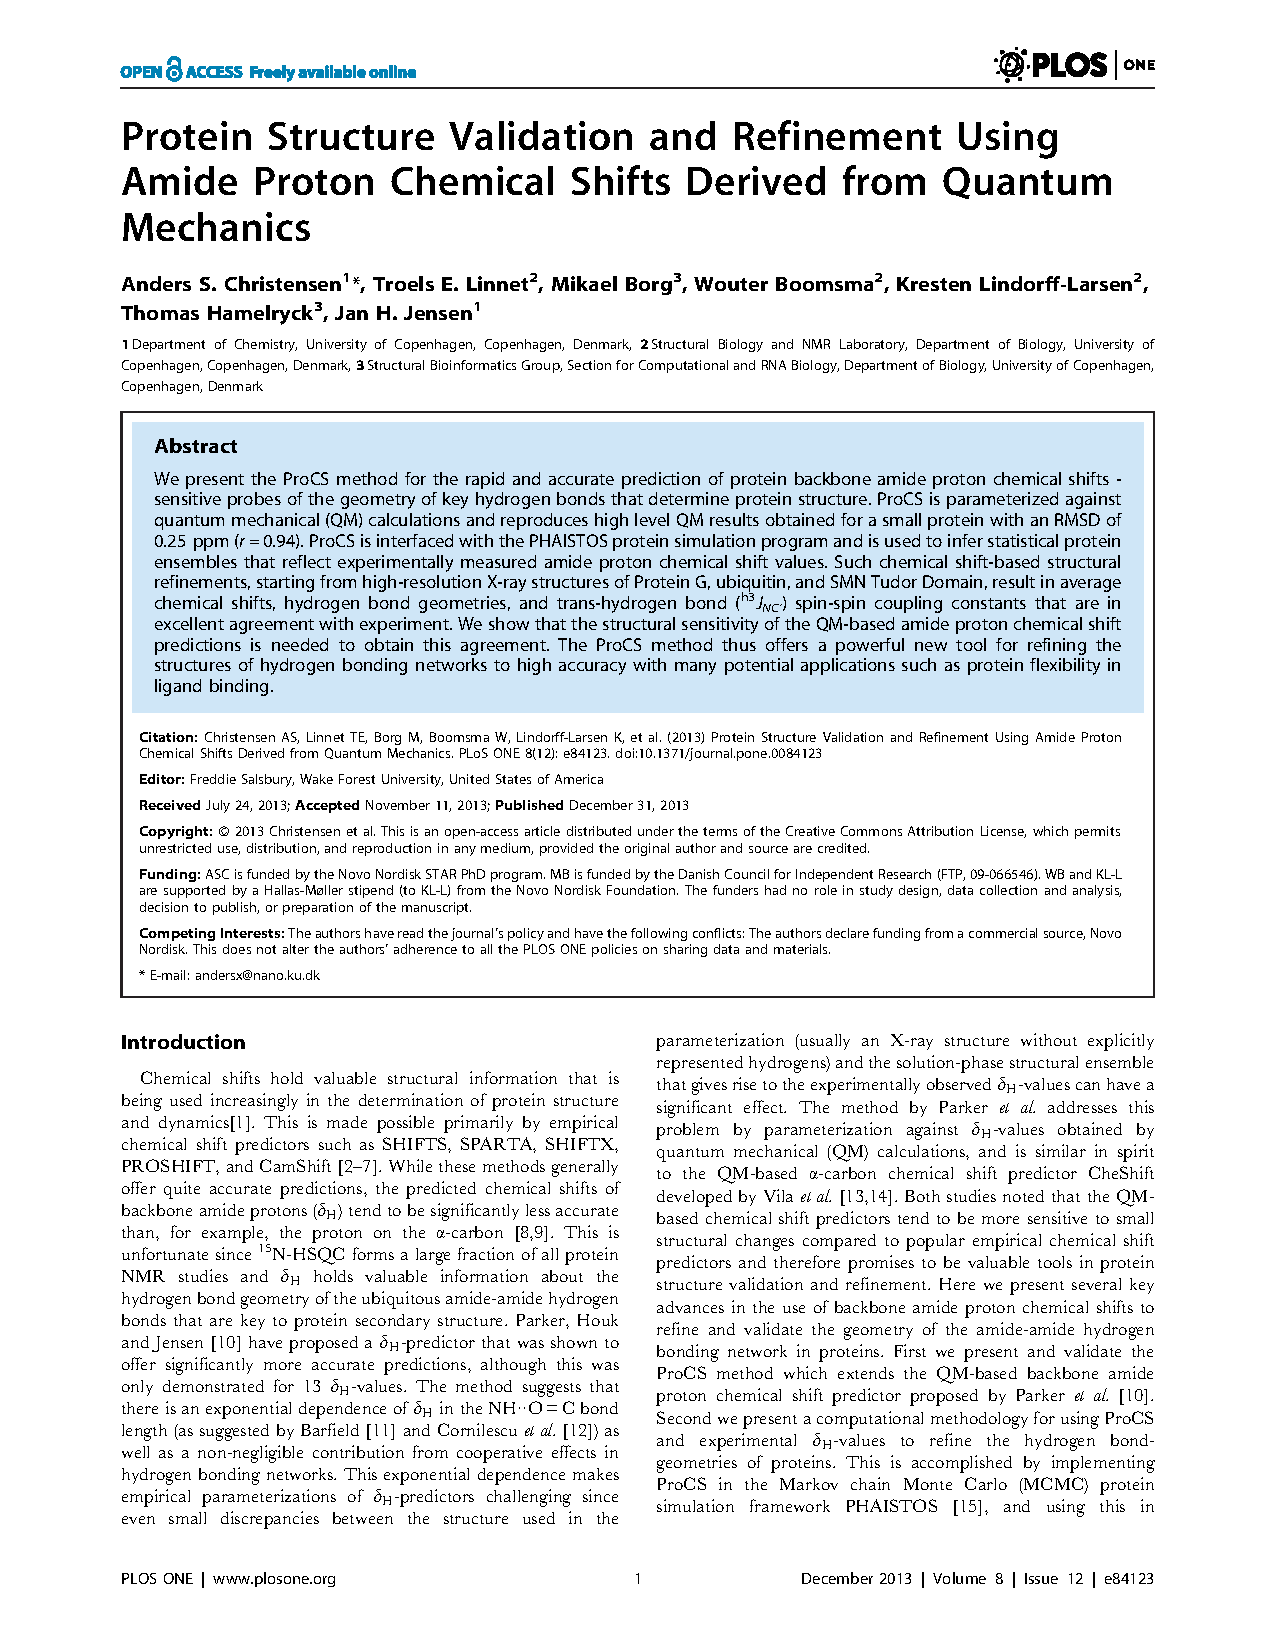
\includepdf[pages={1-10}]{papers/journal_pone_0084123.pdf}

\subsubsection{FragBuilder: An efficient Py    thon library to setup quantum chemistry calculations on peptides models}
\underline{Anders S. Christensen}, Thomas Hamelryck, Jan H. Jensen (2014) FragBuilder: An efficient Python library to setup quantum chemistry calculations on peptides models. \textit{PeerJ} 2:e277.
This paper presents the FragBuilder Python API, which we developed to set up calculation of nearly 2,000,000 QM calculation in the development of ProCS.

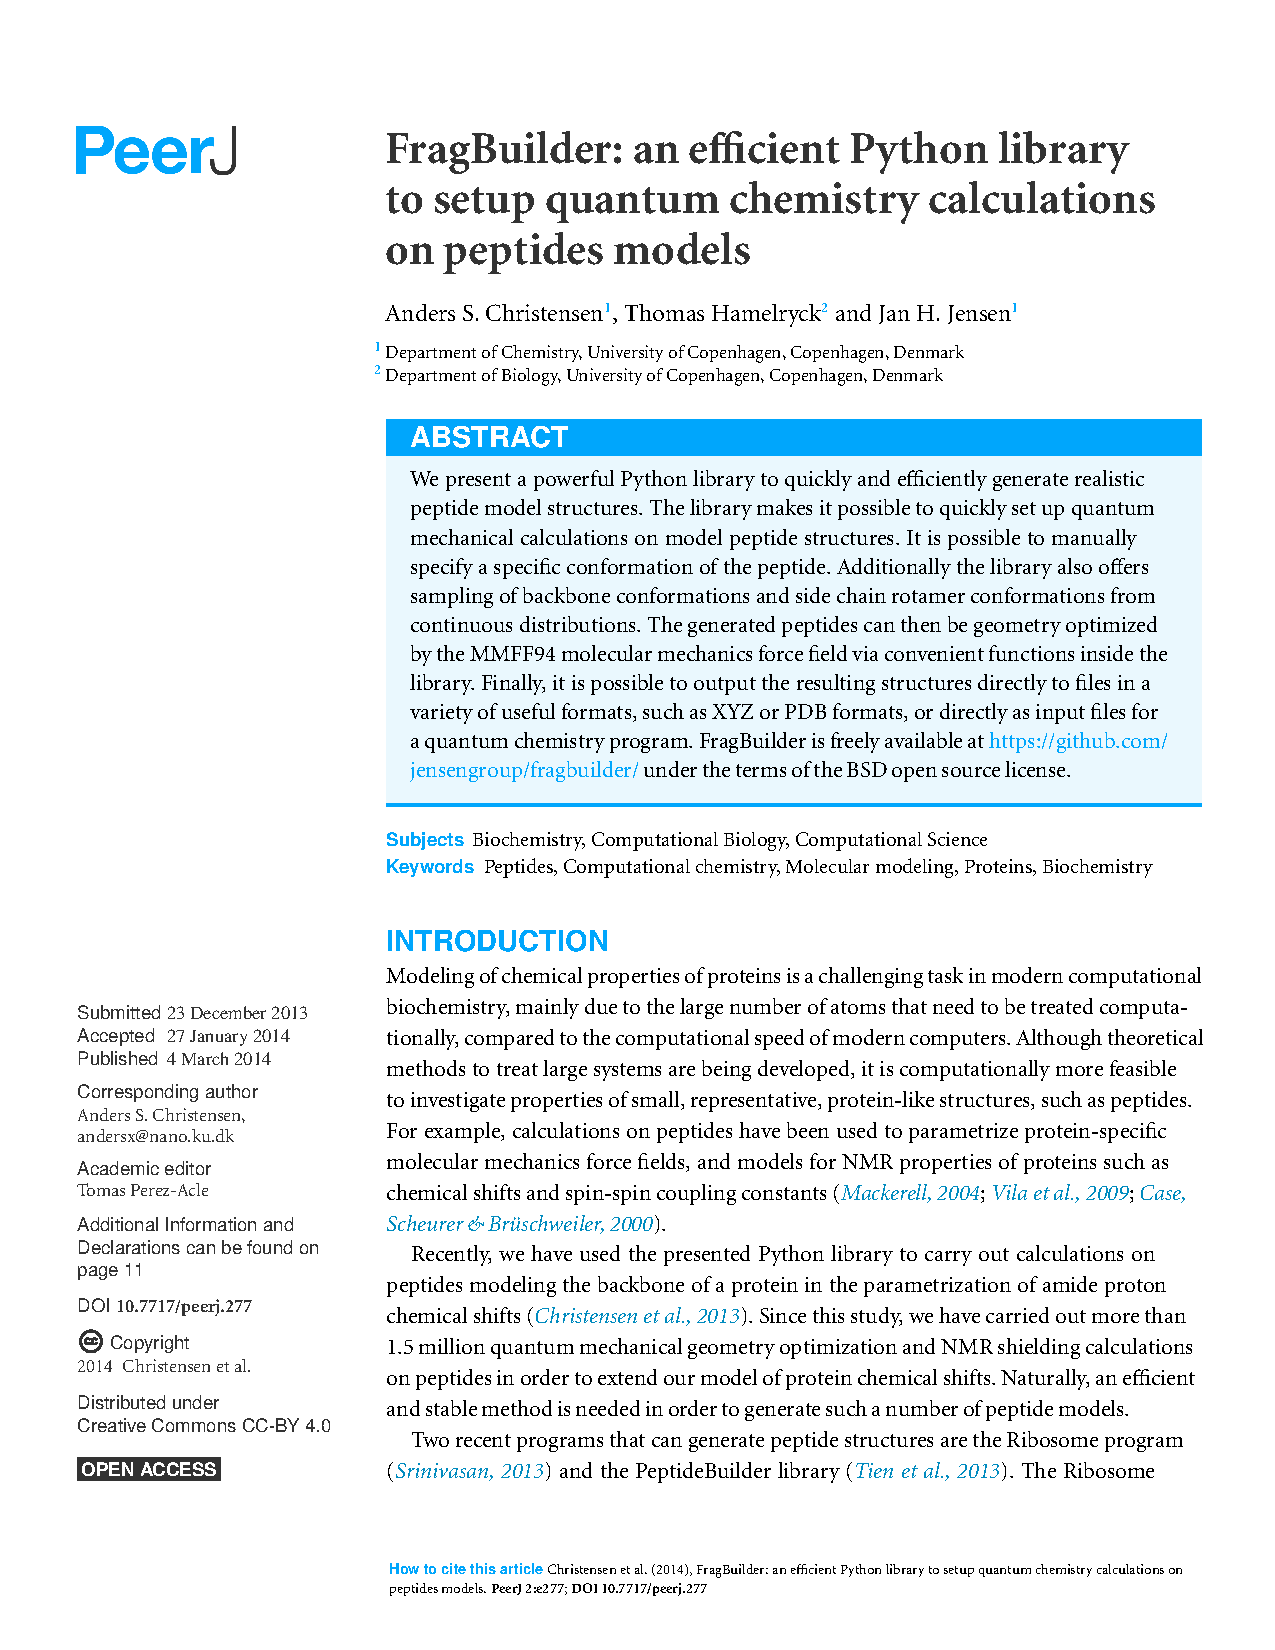
\includepdf[pages={1-13}]{papers/peerj-277.pdf}

%     \item \underline{Anders S. Christensen}, Lars Bratholm, Simon Olsson, Thomas Hamelryck, Jan H. Jensen (2014) Weighting of chemical shift evidence in Monte Carlo simulation of proteins. \textit{ShareLatex} (unpublished).
%     \item Torus-DBN-CS-LARS
%     \item J-coupling Casper/Kongen
% \end{enumerate}
